\chapter{Prochaines étapes}\label{chap:next_steps}
\section{Comptage}\label{anal:comptage}
\paragraph{} Le comptage des animaux traversant le tunnel est la tâche principale pour laquelle ce projet a été mis sur pieds. Maintenant que nous avons des résultats probants pour l'object detection, l'étape suivante consiste en la mise en oeuvre d'une stratégie permettant de compter le nombre de tritons et grenouilles-crapauds traversant le tunnel. Ceci est une tâche assez complexe dans la mesure où une fois les capteurs enclenchés, une série d'images est prise. De ce fait plusieurs images par exemple de tritons à différentes positions peuvent représenter le passage d'un même triton. Pour pallier cette difficulté, nous avons pensé à regrouper les images par prise. Les prises ont été séparées entre elles par un intervalle de 2s afin de réduire au plus la probabilité de compter plusieurs fois le même animal. 

\paragraph{} Une fois les animaux détectés par notre modèle, nous allons procéder à leur comptage. En d'autres termes, nous allons commencer par compter les animaux par images, puis regrouper les détections par prise. Par la suite, nous n'allons conserver pour chaque prise et pour animal, que le nombre maximal de ses occurences comptées sur les images de cette prise. Ce nombre in fine va représenter le nombre d'animaux de ce type pour cette prise. 

\section{Comparaison avec le cahier des charges}

\paragraph{} Lors de l'élaboration du cahier des charges de ce projet, nous avons fixé un certain nombre d'objectifs que nous souhaitions atteindre. Ces objectifs sont divisés en deux grandes catégories, à savoir les "must have" et les "nice to have". Chacune de ces catégories contient trois objectifs distincts, et on va détailler ci-dessous dans quelle mesure ces différents objectifs ont été atteints ou à l'inverse ont échoué.

\subsection{Must have}
\paragraph{} Il s'agit des objectifs à atteindre obligatoirement avant la fin du projet dans la mesure du possible.

\subsubsection{Dessiner une bounding box autour des tritons}
\paragraph{} Comme on peut le constater dans la partie \ref{anal:evaluation}, les deux modèles obtiennent des résultats très différents concernant les tritons. En effet, le modèle RetinaNet est malheureusement incapable de détecter le moindre triton sur les images. En revanche, le modèle Faster R-CNN obtient un AP score plutôt correct de 42.58 sur les tritons. Comme nous avons choisi ce dernier modèle en tant que modèle final, on peut considérer que ce premier objectif obligatoire est atteint.

\subsubsection{Compter les tritons}\label{anal:tritons}
\paragraph{} Comme expliqué dans la section \ref{anal:comptage}, le comptage des tritons et plus globalement des animaux en général s'est avéré être une tâche plus complexe que prévu initialement. En effet, même si cette tâche peut sembler en apparence relativement simple une fois les animaux détectés sur les images, plusieurs problèmes explicités dans le chapitre \ref{anal:comptage} sont intervenus et nous ont malheureusement empêché d'atteindre cet objectif.

\subsubsection{Détecter les crapauds-grenouilles indépendamment des tritons}
\paragraph{} Comme on peut le constater dans la partie \ref{anal:evaluation}, les deux modèles obtiennent des résultats relativement similaires quant à la détection des crapauds-grenouilles sur les images. En effet, ils obtiennent tous les deux un AP score situé entre 40 et 50. Le modèle RetinaNet est toutefois légèrement meilleur puisqu'il parvient à obtenir un AP score de 49.40, contre seulement 42.03 pour Faster R-CNN. Cependant, comme expliqué ci-dessus, RetinaNet ne détecte aucun triton et nous avons donc préféré Faster R-CNN pour notre modèle final. Toujours est-il que le résultat obtenu par Faster R-CNN sur les crapauds-grenouilles reste plutôt satisfaisant et on peut donc considérer que ce troisième objectif est une réussite.

\subsection{Nice to have}
\paragraph{} Il s'agit des objectifs qu'il serait intéressant d'atteindre si le temps le permet mais qui sont d'importance secondaire.

\subsubsection{Distinguer les tritons, les crapauds et les grenouilles}
\paragraph{} Même si la formulation n'est pas très explicite, l'objectif ici était surtout de distinguer les crapauds des grenouilles puisque la distinction entre les tritons et les crapauds-grenouilles était déjà sous-entendue par le dernier objectif "must have". Hélas, cet objectif est un échec puisque dans notre modèle final décrit dans la section \ref{anal:final_model}, nous avons gardé la catégorie crapaud-grenouille en raison des difficultés rencontrées pour différencier ces deux animaux. En effet, les différences entre ces deux espèces sont minimes et même pour un être humain, il est difficile de les distinguer sans être un expert. La marche était donc tout simplement trop haute pour nos réseaux de neurones.

\subsubsection{Compter le nombre de tritons, crapauds et grenouilles qui ont traversé le tunnel dans une période donnée}
\paragraph{} Cet objectif était en quelque sorte le prolongement de l'objectif "must have" détaillé dans la partie \ref{anal:tritons}. Cet objectif initial n'ayant pas pu être atteint, nous n'avons par conséquent pas pu faire aboutir sa version améliorée pour les mêmes raisons. Sans entrer dans les détails de ces raisons qui sont expliqués ci-dessus, cet objectif peut donc être considéré comme un nouvel échec.

\subsubsection{Déterminer le sens de la traversée d’un animal}
\paragraph{} Cet objectif était pertinent principalement pour compter le nombre d'animaux qui traversent les tunnels dans chaque sens. Comme nous n'avons pas été en mesure d'atteindre l'objectif de comptage explicité ci-dessus, nous n'avons pas vraiment essayé de déterminer le sens de la traversée des animaux. De plus, au vu des difficultés rencontrées pour distinguer les crapauds des grenouilles, cette tâche aurait probablement été un peu trop difficile par rapport au bénéfice rapporté par la connaissance du sens de traversée. On peut donc considérer que cet objectif n'a pas été atteint ni même commencé.

\section{Expériences futurs}
Comme dit dans la section \ref{ch:eval:sex:problem}, nous avons remarqué que les animaux sur les côtés de l'image sont souvent mal détectés. Nous avons pensé à deux expériences permettant de possiblement résoudre ce problème: faire une correction non linéaire de la luminosité comme illustré en figure \ref{fig:gamma_correction} et observer après traitements les scores. Il est selon nous nécessaire que la correction soit non linéaire afin de ne pas saturer les zones claires, car il s'agit du centre de l'image, où passent de nombreux animaux.
\begin{figure}[H]
\centering
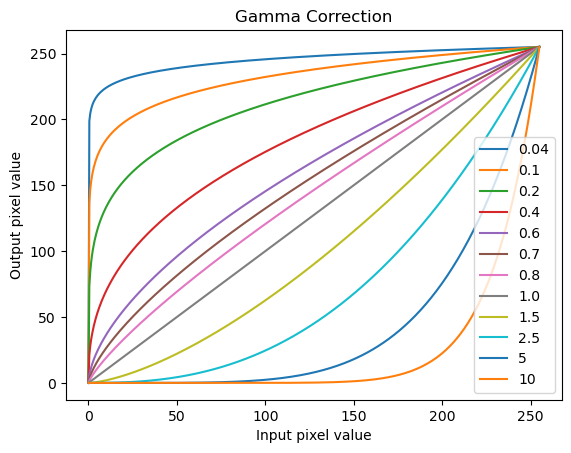
\includegraphics[width=0.5\textwidth]{images/gamma_correction.png}
\caption{Correction non linéaire de la luminosité $O = \displaystyle{\left( \frac{I}{255} \right)^\gamma255}$}
\label{fig:gamma_correction}
\end{figure}

\paragraph{}
Une seconde options que nous n'avons, elle non plus, pas eu le temps de mettre en oeuvre est l'utilisable d'une Grad-Cam afin de détecter les régions d'intérêts sur les images. Cette méthode permet de détecter les régions d'intérêt sur les images et de les mettre en évidence. Nous pensons que cela permettrait de savoir si les côtés sont \textit{observé} par le modèle.

\paragraph{Analyse de la sensibilité}
Une expérience que nous aurions voulu faire est une technique inspirée de la data augmentation. Il s'agit d'occulter des parties de la bounding box afin de voir les parties de l'objet qui déclenche une détection par le modèle.
\paragraph{Let's zoom} La grosse différence entre les classes présentes sur COCO, le dataset d'entrainement originel, et notre dataset de fine-tuning est la taille des objets. En effet, les animaux que nous avons sont beaucoup plus petits que ceux du dataset COCO, ainsi nous aimerions savoir si faire la prédiction en deux étapes : d'abord sur l'image entière puis une seconde fois sur un zoom de la zone prédite permettrait d'améliorer les scores.

\paragraph{Bootstrapping} Vu que nos modèles se trompent rarement, en effet l'erreur la plus commune et la non détection, il serait intéressant d'essayer de les entrainer depuis $0$ en utilisant un plus gros dataset, annoté par la version précédente du modèle! Cela permettrait de voir si le modèle apprend mieux et si les scores augmentent.

\paragraph{Resizing} Durant notre périple, nous avons exploré différents modèles. Pour la plupart d'entre eux, la taille des images demandée en entrée était de 300*300, 500*500 pour SSD, 512*512 YOLOv5 - Cas des images carrées. Les deux modèles précités pour plusieurs raisons dont celle de la taille des entrées constituent des échecs dans notre projet. Car nous rappelons que nous travaillons avec des images de taille 1920*1080. Nous pensons donc que pour de futures expériences, il serait intéressant de redimensionner les images pour permettre que celles ci non seulement s'adaptent à plusieurs modèles, mais aussi pour accélérer le temps de traitement. Passer d'une taille d'image de 1920*1080 à une taille de 300*300 par exemple ne constitue pas pour la tâche que nous faisons une perte d'informations handicapante. À confirmer avec une expérience. 
